\documentclass[11pt]{article}
\renewcommand{\baselinestretch}{1.05}
\usepackage{amsmath,amsthm,verbatim,amssymb,amsfonts,amscd, graphicx}
\usepackage{graphics}
\topmargin0.0cm
\headheight0.0cm
\headsep0.0cm
\oddsidemargin0.0cm
\textheight23.0cm
\textwidth16.5cm
\footskip1.0cm
\theoremstyle{plain}
\newtheorem{theorem}{Theorem}
\newtheorem{corollary}{Corollary}
\newtheorem{lemma}{Lemma}
\newtheorem{proposition}{Proposition}
\newtheorem*{surfacecor}{Corollary 1}
\newtheorem{conjecture}{Conjecture} 
\newtheorem{question}{Question} 
\theoremstyle{definition}
\newtheorem{definition}{Definition}

\usepackage{graphicx}


 \begin{document}

\title{Homework 6 Machine Learning}
\author{Marco Treglia}
\date{}
\maketitle

\section{Bayesian Network}
Bayes network: a directed acyclic graph defining a joint probability distribution over a set of variables
Each node denotes a random variable.Each node is conditionally independent of its non-descendents, given its immediate parents.A conditional probability distribution (CPD) is associated with each node N, defining P(N | Parents(N))

\section{Assignment 1}
\begin{center}
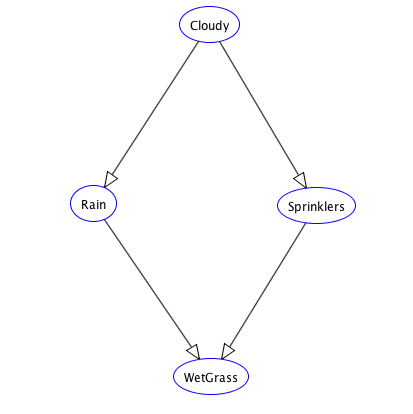
\includegraphics[scale=0.3]{0}
\end{center}

\subsection{Joint probability function}
$$P(c,r,s,w) = P(c) \cdot P(r | c) \cdot P(s | c ) \cdot P(w | r ,s ) $$
\subsection{Joint probability function}
\begin{center}
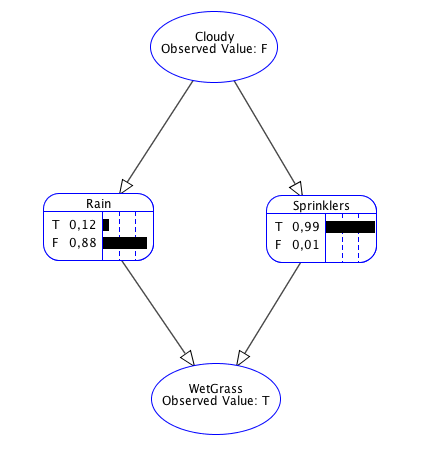
\includegraphics[scale=0.4]{1}
\end{center}

\section{Assignment 2}

\begin{center}
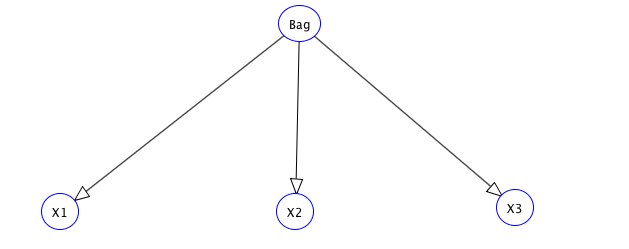
\includegraphics[scale=0.3]{3}
\end{center}




\begin{center}
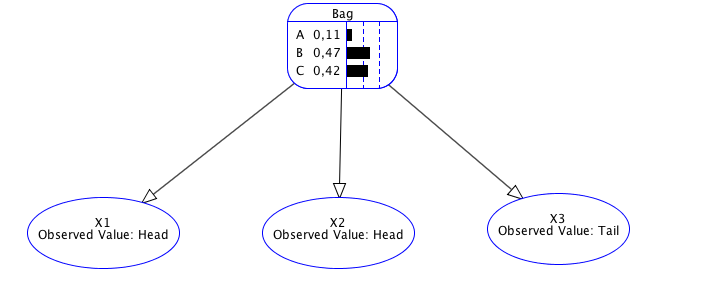
\includegraphics[scale=0.4]{2}
\end{center}

\section{Assignment 3}

\begin{center}
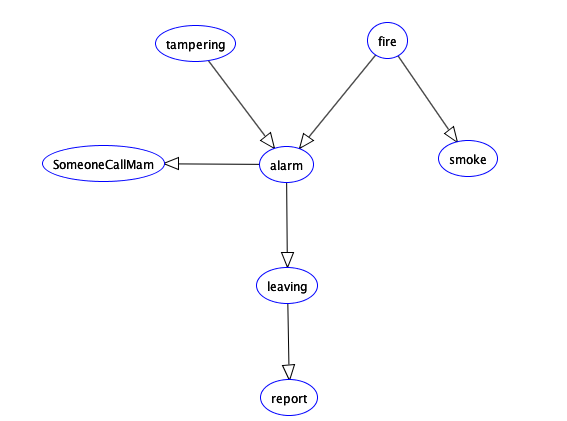
\includegraphics[scale=0.5]{4}
\end{center}

\subsection{Joint probability function}
$$P(t,f,a,s,l,r) = P(t) \cdot P(f) \cdot P(a | t, f) \cdot P(s | f ) \cdot P(l | a ) \cdot P(r | l)$$

\subsection{Node Call}
\begin{center}
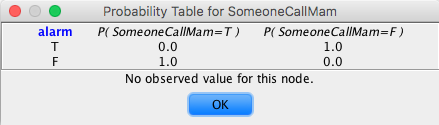
\includegraphics[scale=0.4]{5}
\end{center}


\end{document}